\chapter{Background and Theory}
%This chapter should describe the theoretical background needed to understand and solve the problem. 
%For instance, a description of the hardware platform or specific components involved in this assignment, definition of concepts that are important to understand the solution should be summarized here.
%Add citations to show sources whenever appropriate, LaTeX and bibliography managers make this easy. For instance, ``I always thought something was fundamentally wrong with the universe'' \cite{adams1995hitchhiker}.


%%%%%%%%%%%%%%%%%%%%%%%%%%%%%%%%%%%%%%%%%%%%%%%%%%%%%%%%%%%%%%%%%%%%%%%%%
\section{RSA encryption/decryption}
RSA has its name from the creators; Ron Rivest, Adi Shamir and Len Adleman. RSA uses two different keys. One for encryption (public key); the other is for decryption (private key). \\
This is an asymmetric algorithm, with the important advantage that anyone can encrypt a message for the receiver (using the public part of the key pair), but only the receiver (who has the private key) can decrypt and read it. The method relies on a one-way function f such that it is easy to compute $Y=f(X)$, but (practically) impossible to compute $X=f_1(Y)$, unless you have the correct key $k$.
\\
RSA is widely used in electronic commerce protocols (banking, online shopping and such), and is believed to be secure, given sufficiently long keys and the use of up-to-date implementations. As of 2016 the recommended key length is minimum 2048 bits for a good balance between speed and security.

\begin{figure}[H]
\centering
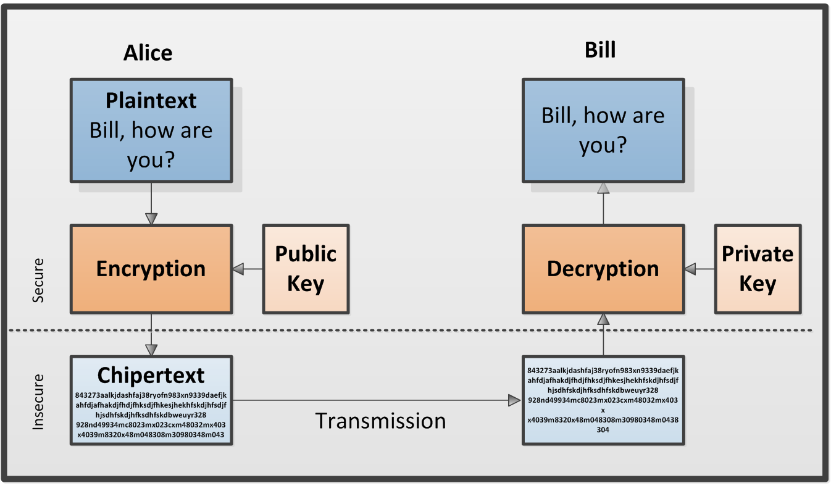
\includegraphics[width=0.7\textwidth]{images/rsa.PNG}
\caption{RSA encryption/decryption mechanism}
\label{fig:rsa}
\end{figure}

The same computation is performed for encryption and decryption, but with different parameters. The encryption and decryption keys (d,e) are related through the following equation:\\
Encryption: (public key: {e,n})
\begin{equation}
    C=M^e mod n, M<n
\end{equation}
Decryption:(private key: {d,n})
\begin{equation}
    M=C^d mod n = (M^e)^d mod n
\end{equation}

Appropriate values for e,d, and n can be found using Euler's theorem.


%%%%%%%%%%%%%%%%%%%%%%%%%%%%%%%%%%%%%%%%%%%%%%%%%%%%%%%%%%%%%%%%%%%%%%%%%%%%%%
\section{Methods for computing $M^emod(n)$}
Modular exponentiation is achieved by replacing all multiplications in the algorithm by modular multiplications.
The computation of $M^e(mod(n))$ is called modular exponentiation. In the exponentation process for the RSA algorithm, we know the exponent (e) and the modulus (n) in advance but not the base (M). 
The modular exponentiation can be broken into a series of modular multiplications and modular squaring operations.

Computing $C:= M^e (mod(n))$ by first exponentiation and then performing a division to obtain the remainder $C:=(M^e)\%n $ would have resulted in an enormous space requirement. Assuming, M and e have 128 bits each, we need
\begin{equation}
    log_2(M^e)=e*log_2(M) = 2^{128}*128=2^{135} = 10^{40}
\end{equation}
bits in order to store $M^e$.

The naive method of computing a modular multiplication requires e-1 modular multiplications. However not all power of M need to be computed. Using squerings you can reduce the number of multiplications. This method is called the binary method or square and multiply method.
The binary method for computing $M^emodn$ given the integers M, e, and n has two variations depending on the direction by which the bits of e are scanned: Left-to-Right(LR) and Right-to-Left(RL).

\begin{algorithm}
\setAlgoLined
    \textbf{LR Binary Method}\\
    Input: M, e, n\\
    Output: C:= M^e mod n\\
    1. if $e_{n-1}=1$ then $C:=M$ else $C:=1$\\
    2. for $i=h-2$ downto 0\\
    2a.\quad $C:=C * C (mod n)$\\
    2b.\quad if $e_{i}=1$ then $C:=C * M (mod n)$\\
    3. return $C$
\end{algorithm}

The bits of e are scanned from the most significant to the least significant, and a modular squaring is performed for each bit. A modular multiplication operation is performed only if the bit is 1.

\subsection{Modular Multiplication}
There are four approaches for computing P= AB (mod n) in hardware.\cite{rsahardware}\\
\begin{itemize}
  \item Multiply and then Reduce:First multiply $t:=a*b$. Here t is a 2k-bit or 2s-word number. The reduction is accomplished by dividingt t by n, and we obtain the reminder.
  \item The steps of the multiplication and reduction are interleaved (Blakley's method).
  \item Brickell's method.
  \item Montgomery's method: This algorithm rearranges the residue class modulo n, and uses module $2^j$ arithmetic.
\end{itemize}

\subsubsection{Blakley's Method}
Computes $a*b mod n$ by interleaving the shift-add steps of the multiplication and the shift-substract steps of the division. This is a bit-by-bit multiplication algorithm.

\begin{algorithm}
The Blakley Algorithm\\
Input: a,b,n\\
Output: R = a * b mod n\\
1. $R:= 0$\\
2. for $i=0$ to $k-1$ \\
3. $R:=2R + a_{k-1-i}*b$\\
4. $R:= R mod n$\\
5. return $R$
\end{algorithm}

This algorithm computes the remainder R in k steps, where at each step one addition, and at most two substractions are performed.


%%%%%%%%%%%%%%%%%%%%%%%%%%%%%%%%%%%%%%%%%%%%%%%%%%%%%%%%%%%%%%%%%%%%%%%%%%%%
\subsubsection{Montgomery's Method}
Montgomery's algorithm is an efficient way of doing modular multiplication. This algorithm works extremly well when implemented on general-purpose computers (signal processors or microprocessors) which are capable of performing fast arithmetic modulo a power of 2. 

This algorithm replaces the division-by-n operation with division by a power of 2. This operation is easily accomplished on a computer since the numbers are represented in binary form\cite{highspeedrsa}, and one only needs to shift the number $log(n)$ places to right.

The Montgomery product is defined as
\begin{equation}
    \bar{R}= \bar{a} * \bar{b} * r^{-1} mod n
\end{equation}
where $r^{-1}$ is the inverse of r module n
\begin{equation}
    r^{-1}*r = 1 mod n
\end{equation}
The resulting number $\bar{R}$ is the n-residue of the product
\begin{equation}
    R= a * b * mod (n)
\end{equation}
In order to describe the Montgomery reduction algorithm, we need an additional quantity, n', which is the integer wit the property 
\begin{equation}
    r * r^{-1} - n * n' =1
\end{equation}
The Montgomery algorithm computes
\begin{equation}
    MonPro(A,B) = A * B * r^{-1}mod n
\end{equation}

We take $r=2^k$ and assume that the number of bits in A or B is less than k. The product $u = A * B * 2^{-k}(mod n)$ can be compute by the following binary add-shift algorithm:\\
\begin{algorithm}[H]

    1. u:=0\\
    2. for i= 0 to k-1\\
    2a.\quad u:=u + A_i * B\\
    2b.\quad if u is odd then u:=u+n\\
    2c.\quad u:=u/2\\
\end{algorithm}
The most important feature of the Montgomery product algorithm is that the operations involved are multiplications modulo r and divisions by r, both of which are intrinsically fast operations since r is a power of 2 \cite{highspeedrsa}.


\subsection{Montgomery Exponentiation}
One can use the montgomery product algorithm to when several modular multiplications with the same modulus are needed, for instance when we need to compute $M^e mod n$. One can use one of the addition chain algorithm to replace the exponentiation with a series of multiplication and squaring modular operations. Using the binary method for the exponentiation we then have:

\begin{algorithm}
function ModExp(M,e,n){n is an odd number}\\
Step 1. Compute n' using the extended Euclidean algorithm.\\
Step 2. $\bar{M} := M* r mod n\\
Step 3. \bar{x}:= 1* r mod n$\\
Step 4. for $i=k-1$ downto $0$ do\\
Step 5. \quad $\bar{x}= MonPro(\bar{x},\bar{x})$\\
Step 6. \quad if $e_i =1$ then $\bar{x}:= MonPro(\bar{M}, \bar{x})$\\
Step 7. $x:= MonPro(\bar{x},1)$\\
Step 8. return $x$\\
\end{algorithm}

%%%%%%%%%%%%%%%%%%%%%%%%%%%%%%%%%%%%%%%%%%%%%%%%%%%%%%%%%%%%%%%%%%%%%%%%%%%%%
\section{VHDL}
VHDL (\emph{Very high speed integrated circuits Hardware Description Language}) is a language used for describing and simulating/synthesizing digital logic.\\
It allows for much more efficient design of logic by formulating the desired behavior as a "program", instead of having to draw all the logic gates and connections manually.
VHDL is a hardware description language. The code describes the behavior or structure of an electronic circuit\cite{pedroni}. Its main applications include synthesis of digital cirtuits onto FPGA (Field Programmable Gate Array) or for layout/mask generation for ASIC (Application-Specific Integrated Circuit) fabrication.

VHDL allows for circuit synthesis as well as circuit simulation. Circuit synthesis translates the source code into hardware structure that implements the intended functionality, whil circuit simulation is a testing procedure to ensure correct functionality. 